\documentclass[xcolor=dvipsnames,notes]{beamer}
\usecolortheme[named=Brown]{structure}
\usetheme{default}
\setbeamertemplate{navigation symbols}{} 
\usepackage{tikz}
\usetikzlibrary{arrows,decorations.pathmorphing,backgrounds,positioning,fit}
\usetikzlibrary{datavisualization.formats.functions}
\usetikzlibrary{shapes}
\usetikzlibrary{calc,patterns,angles,quotes}
%     
%Here are some macro's saving time and labour:     
%     
\newcommand{\const}{\mbox{const}}      
\newcommand{\est}{\mbox{{\tiny est}}}      
\newcommand{\im}{\mbox{$\Im \mbox{m}$}}      
\newcommand{\obs}{\mbox{{\tiny obs}}}      
\newcommand{\otherwise}{\mbox{otherwise}}      
\newcommand{\real}{\mbox{$\Re \mbox{e}$}}      
\newcommand{\sign}{\mbox{sign}}      
\newcommand{\sinc}{\mbox{sinc}}      
%
\newcommand{\p}{\mbox{$\partial$}}      
\renewcommand{\d}{\mbox{$\partial$}}      
\newcommand{\w}{\mbox{$\omega$}}      
%
\newcommand{\AAA}{\mbox{\boldmath $A$}}   
\newcommand{\BB}{\mbox{\boldmath $B$}}     
\newcommand{\CC}{\mbox{\boldmath $C$}}     
\newcommand{\DD}{\mbox{\boldmath $D$}}     
\newcommand{\EE}{\mbox{\boldmath $E$}}     
\newcommand{\FF}{\mbox{\boldmath $F$}}   
\newcommand{\GG}{\mbox{\boldmath $G$}}   
\newcommand{\HH}{\mbox{\boldmath $H$}}   
\newcommand{\II}{\mbox{\boldmath $I$}}   
\newcommand{\JJ}{\mbox{\boldmath $J$}}   
\newcommand{\KK}{\mbox{\boldmath $K$}}   
\newcommand{\LL}{\mbox{\boldmath $L$}}   
\newcommand{\MM}{\mbox{\boldmath $M$}}   
\newcommand{\NN}{\mbox{\boldmath $N$}}   
\newcommand{\OO}{\mbox{\boldmath $O$}}   
\newcommand{\PP}{\mbox{\boldmath $P$}}   
\newcommand{\QQ}{\mbox{\boldmath $Q$}}   
\newcommand{\RR}{\mbox{\boldmath $R$}}   
\newcommand{\SSS}{\mbox{\boldmath $S$}}   
\newcommand{\TT}{\mbox{\boldmath $T$}}   
\newcommand{\UU}{\mbox{\boldmath $U$}}   
\newcommand{\VV}{\mbox{\boldmath $V$}}   
\newcommand{\WW}{\mbox{\boldmath $W$}}   
\newcommand{\XX}{\mbox{\boldmath $X$}}   
\newcommand{\YY}{\mbox{\boldmath $Y$}}   
\newcommand{\ZZ}{\mbox{\boldmath $Z$}}   
%
%\newcommand{\aaa}{\mbox{\boldmath $a$}}     
\newcommand{\bb}{\mbox{\boldmath $b$}}     
\newcommand{\cc}{\mbox{\boldmath $c$}}     
\newcommand{\dd}{\mbox{\boldmath $d$}}     
\newcommand{\ee}{\mbox{\boldmath $e$}}   
\newcommand{\ff}{\mbox{\boldmath $f$}}   
%\newcommand{\ggg}{\mbox{\boldmath $g$}}   
\newcommand{\hh}{\mbox{\boldmath $h$}}   
\newcommand{\ii}{\mbox{\boldmath $i$}}   
\newcommand{\jj}{\mbox{\boldmath $j$}}   
\newcommand{\kk}{\mbox{\boldmath $k$}}   
%\newcommand{\lll}{\mbox{\boldmath $l$}}   
\newcommand{\mm}{\mbox{\boldmath $m$}}   
\newcommand{\nn}{\mbox{\boldmath $n$}}   
\newcommand{\pp}{\mbox{\boldmath $p$}}   
\newcommand{\qq}{\mbox{\boldmath $q$}}   
\newcommand{\rr}{\mbox{\boldmath $r$}}   
%\newcommand{\sss}{\mbox{\boldmath $s$}}   
%\newcommand{\ttt}{\mbox{\boldmath $t$}}   
\newcommand{\uu}{\mbox{\boldmath $u$}}   
\newcommand{\vv}{\mbox{\boldmath $v$}}   
\newcommand{\ww}{\mbox{\boldmath $w$}}   
\newcommand{\xx}{\mbox{\boldmath $x$}}   
\newcommand{\yy}{\mbox{\boldmath $y$}}   
\newcommand{\zz}{\mbox{\boldmath $z$}}   
%
\newcommand{\balpha}{\mbox{\boldmath $\alpha$}}     
\newcommand{\bpsi}{\mbox{\boldmath $\psi$}}     
\newcommand{\bphi}{\mbox{\boldmath $\phi$}}     
\newcommand{\bbeta}{\mbox{\boldmath $\beta$}}     
\newcommand{\btheta}{\mbox{\boldmath $\theta$}}     
\newcommand{\bdelta}{\mbox{\boldmath $\delta$}}     
\newcommand{\bgamma}{\mbox{\boldmath $d$}}     
\newcommand{\bGamma}{\mbox{\boldmath $\Gamma$}}     
\newcommand{\bLambda}{\mbox{\boldmath $\Lambda$}}     
\newcommand{\bmu}{\mbox{\boldmath $\mu$}}     
\newcommand{\bnabla}{\mbox{\boldmath $\nabla$}}     
\newcommand{\brho}{\mbox{\boldmath $\rho$}}     
\newcommand{\bSigma}{\mbox{\boldmath $\Sigma$}}     
\newcommand{\bsigma}{\mbox{\boldmath $\sigma$}}     
\newcommand{\bxi}{\mbox{\boldmath $\xi$}}     
\newcommand{\bepsilon}{\mbox{\boldmath $\epsilon$}}     
\newcommand{\blambda}{\mbox{\boldmath $\lambda$}}     
\newcommand{\BLambda}{\mbox{\boldmath $\Lambda$}}     
%-------------------------------------%
%  \Appendix - a new appendix command %
%-------------------------------------%
%The appendix command is used as in
% \Appendix{A}{The wave equation as a matrix equation}
\newcommand {\Appendix}[1]{
              \section*{APPENDIX #1}
              \setcounter{equation}{0}
              \renewcommand{\theequation} 
              {A-\arabic{equation}}}
\newcommand {\Appendices}[2]{
              \section*{APPENDIX #1: #2 }
              \setcounter{equation}{0}
              \renewcommand{\theequation} 
              {#1-\arabic{equation}}}
%------------------------------------%
%    \aref - a new cite command.     % 
%------------------------------------%
\newcommand{\aref}[2]{\nocite{#1}#2} 
%----------------------------------------
%\eqref -an equation reference command
%----------------------------------------
%\newcommand{\eqref}[1]{(\ref{#1})}
%\newcommand{\eqref}[1]{\ref{#1}}

\usepackage{epsfig}
\usepackage{natbib}
\usepackage{graphicx}
\usepackage{multimedia}
\usepackage{verbatim}
\include{acmmacro}
\begin{document}
%\setbeamercolor{titlelike}{fg=gray,bg=white}
%\setbeamercolor{itemize item}{fg=gray,bg=white}
%\setbeamercolor{enumerate item}{fg=gray,bg=white}
%\setbeamercolor{block title}{fg=black,bg=white}
%==============================================
\title{TPG4190 Seismic data acquisition and processing \\
               Lecture 20: Deconvolution}
\author{B. Arntsen}
\institute[NTNU]{
  NTNU\\
  Department of Geoscience and petroleum \\
  \texttt{borge.arntsen@ntnu.no}
}
\date{Trondheim fall 2020}
\begin{frame}
 \titlepage
\end{frame}
%

%==============================================
\title{Geophysical Analysis - lecture 10} 
\author{B. Arntsen}
\begin{frame}
 \titlepage
\end{frame}
%==============================================
\begin{frame}{Contents}
\sf\Large
\begin{itemize}
  \item 4.1 The convolutional model for seismic data
  \item 4.2 Deconvolution
  \item 4.3 Bandwidth and resolution
\end{itemize}
\end{frame}
%
\begin{frame}{Convolutional model}
\begin{figure}
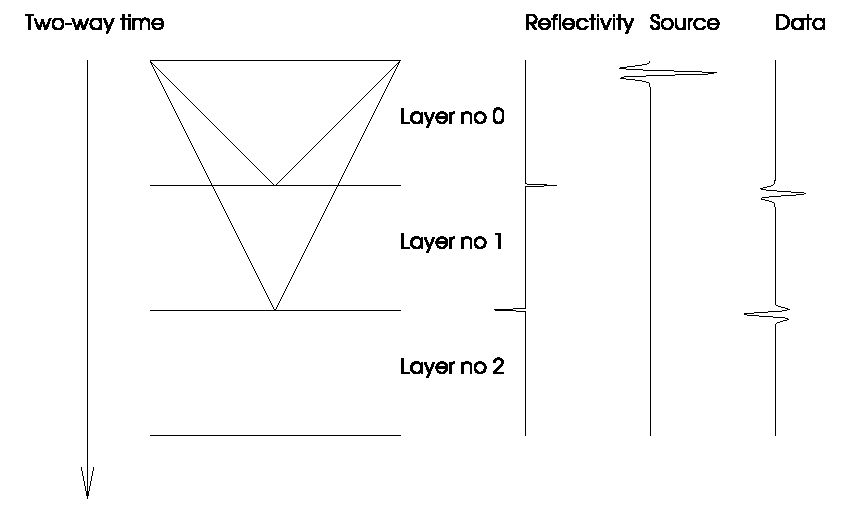
\includegraphics[width=\textwidth]{Fig/layers.pdf}
%\plot{layers}{width=\textwidth}{Layered earth model}
\caption{Layered earth model}
\end{figure}
\end{frame}
%
\begin{frame}{Convolutional model}
\begin{itemize}
 \item vertical propagation
\end{itemize}
%
Reflected signal
\begin{eqnarray}
 a(t)=r_0\frac{s(t-\phi_0)}{2d_0}
\label{eq:3-60}.
\end{eqnarray}
\begin{itemize}
 \item $\phi_0 = 2 d_0/c_0$: two-way traveltime 
 \item $r_0$ : reflection coefficient
 \item $d_0$ : layer thickness
\end{itemize}
\end{frame}
%
\begin{frame}{Convolutional model}
Reflection coefficient defined by
\begin{eqnarray}
 r_0 =\frac{c_1\rho_1-c_0\rho_0}{c_1\rho_1+c_0\rho_0}.
\label{eq:3-61}
\end{eqnarray}
\begin{itemize}
  \item $c_0, c_1$: Wave velocity
  \item $\rho_0, \rho_1$: Density
\end{itemize}
\end{frame}
%
\begin{frame}{Convolutional model}
\begin{itemize}
\item Signal recorded at the surface:
\end{itemize}
%
\begin{eqnarray}
 a(t)=r_0\frac{s(t-\phi_0)}{2d_0} + r_1\frac{s[t-(\phi_0 + \phi_1)]}{2d_0+2d_1},
\label{eq:3-62}
\end{eqnarray}
%
\end{frame}
%
\begin{frame}{Convolutional model}
\begin{itemize}
 \item Neglect spherical spreading
 \item General model
\end{itemize}
%
\begin{eqnarray}
 a(t) = \sum^N_{k=0} r_k s(t-\tau_k),
\label{eq:3-63}
\end{eqnarray}
\begin{itemize}
 \item $\tau_k = \sum^k_{l=0} \phi_l$ two way traveltime to interface no k.
\end{itemize}
\end{frame}
%
\begin{frame}{Convolutional model}
\sf\Large
 \begin{itemize}
  \item $\tau_k=k\Delta t$.
 \end{itemize}
%
\begin{eqnarray}
  a_k = \sum^N_{l=0} r_l s_{k-l},
\label{eq:3-64}
\end{eqnarray}
\begin{eqnarray}
  a_k & = & a(t=k\Delta t)\nonumber,\\
  s_k & = & s(t=k\Delta t).
\end{eqnarray}

Continuous case:
%
\begin{eqnarray}
 a(t)=\int^{+\infty}_{\tau=0} r(\tau)s(t-\tau),
\label{eq:3-65}
\end{eqnarray}
%
\end{frame}
%
\begin{frame}{Convolutional model}
%
\begin{itemize}
  \item Vertical wave propagation
  \item Neglect vertical spreading
  \item Only primary reflections
   \item Earth is a linear filter
   \item $r(t)$ Earth's impulse response
 \end{itemize}
\end{frame}
%
\begin{frame}{Deconvolution}
\begin{itemize}
\item Convolutional model for
\end{itemize}
seismic waves 
%
\begin{eqnarray}
  y(t)=r(t)*s(t),
      \label{eq:cmodel}
\end{eqnarray}
%
\begin{itemize}
\item $s(t)$: seismic source 
\item $r(t)$: reflectivity
\end{itemize}
\end{frame}
%
\begin{frame}{Deconvolution}
\sf\Large
\begin{itemize}
\item Recover $r(t)$ when
\item $s(t)$ given
\item $y(t)$ given
\end{itemize}
\end{frame}
%
\begin{frame}{Spiking deconvolution}
\sf\Large 
\begin{itemize}
  \item Fourier transformation of \eqref{eq:cmodel}
\end{itemize}
%
\begin{eqnarray}
  Y(f) = R(f) S(f)
      \label{eq:cmodel-four}
\end{eqnarray}
%
\begin{itemize}
  \item Solution
\end{itemize}
%
\begin{eqnarray}
  R(f) = \frac{Y(f)}{S(f)}.
      \label{eq:refl}
\end{eqnarray}
\end{frame}
%
\begin{frame}{Deconvolution}
\begin{itemize}
 \item Equation \eqref{eq:refl} slightly reformulated 
\end{itemize}
%
\begin{eqnarray}
  R(f) = S^{-1}(f)Y(f),
      \label{eq:inv}
\end{eqnarray}
%
\begin{itemize}
\item $S^{-1}=1/S(f)$: {\em inverse} filter.
\item
$S^{-1}$ removes the source
\item recovers reflection coefficients
\end{itemize}
\end{frame}
%
\begin{frame}{Deconvolution}
%
\begin{figure}
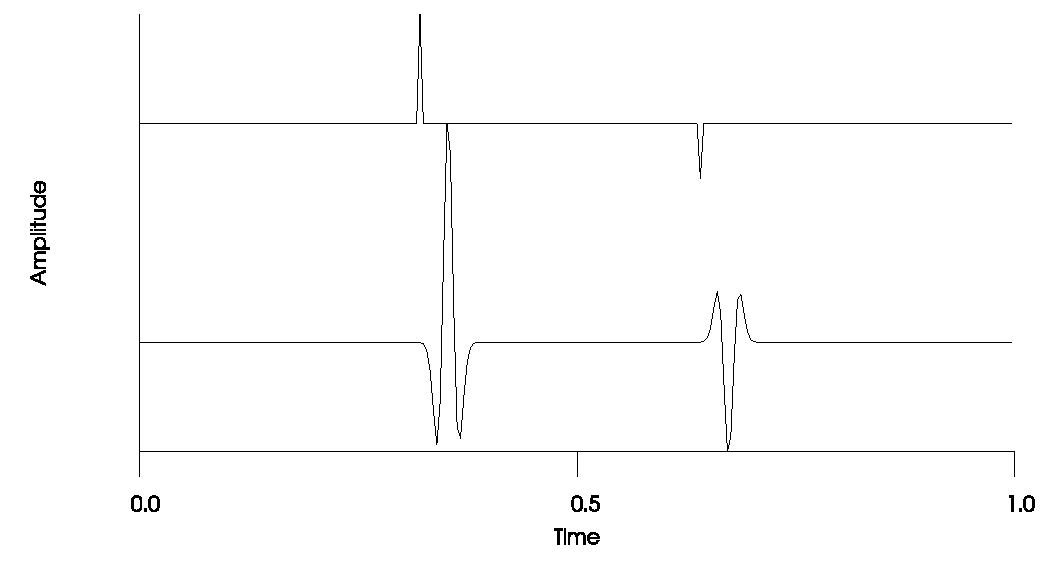
\includegraphics[width=0.8\textwidth]{Fig/fdecon2}
\caption{Spiking decon}
%\plot{fdecon2}{width=0.8\textwidth}{Spiking decon}
\end{figure}
%\begin{figure}[h]
%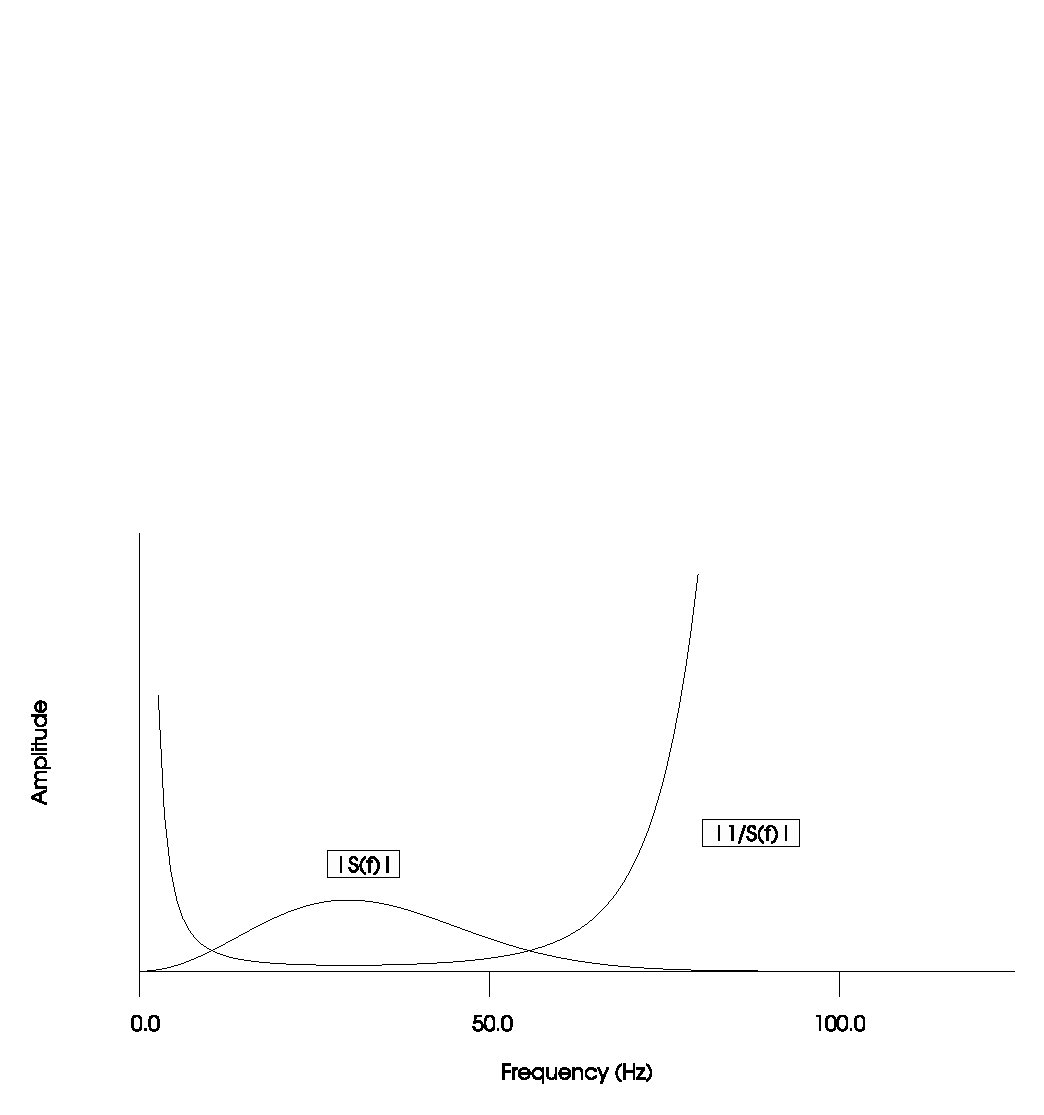
\epsfig{file=../Fig/fdecon.pdf, width=0.6\textwidth}
%\label{fig:fdecon}
%\end{figure}
%
The spectrum of a Ricker pulse and it's inverse
\end{frame}
%
\begin{frame}{Deconvolution}
%\sf\Large
%\begin{figure}[h]
%\epsfig{file=../Fig/fdecon2-spectr.pdf, width=0.8\textwidth}
\begin{figure}
\includegraphics[width=0.8\textwidth]{Fig/fdecon2-spectr}
%\plot{fdecon2-spectr}{width=0.8\textwidth}{Deconvolution spectrum}
\caption{Deconvolution spectrum}
\end{figure}
%\label{fig:fdecon2-spectr}
%\end{figure}
%
The spectrum of the input data $|G(f)|$ and the
         deconvolved output $|R(f)|$.
%
\end{frame}
%
\begin{frame}{Deconvolution}
\sf\Large
%
\begin{figure}[h]
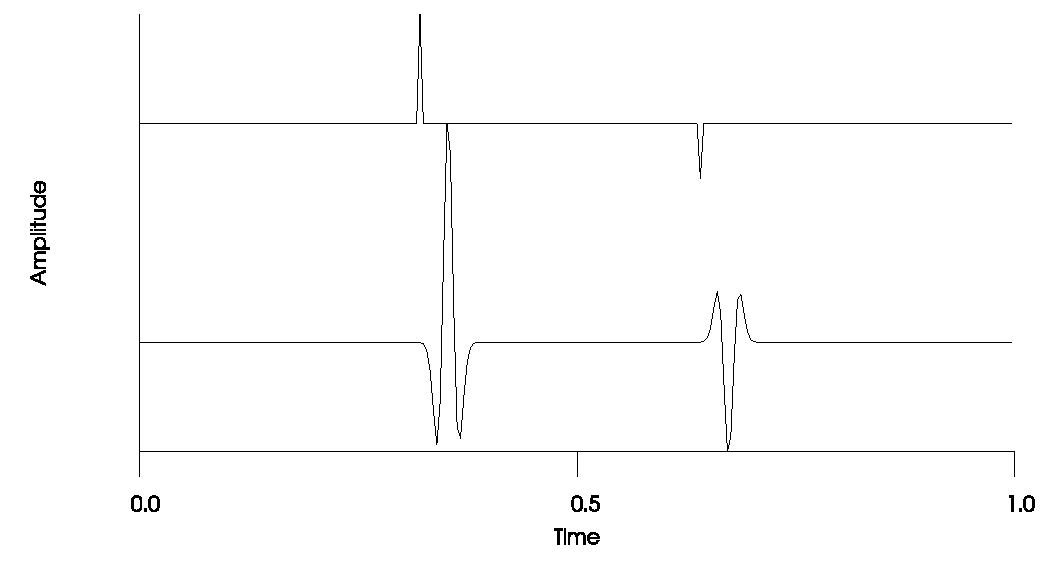
\includegraphics[width=0.8\textwidth]{Fig/fdecon2.pdf}
%\plot{fdecon2}{width=0.8\textwidth}{Deconvolution}
\caption{Deconvolution}
\label{fig:fdecon2}
\end{figure}
\end{frame}
%
\begin{frame}{Deconvolution}
\sf\Large
\begin{itemize}
 \item Real seismic data contains noise
\end{itemize}
%
\begin{eqnarray}
  Y(f) = R(f) S(f) + N(f),
      \label{eq:cmodel-four-noise}
\end{eqnarray}
%
\begin{itemize}
 \item $N(f)$ : White (random) noise
\end{itemize}
%
\begin{eqnarray}
  R(f) = S^{-1}(f) Y(f) - S^{-1}(f)N(f).
      \label{eq:refl-noise}
\end{eqnarray}
%
\end{frame}
%
\begin{frame}{Deconvolution}
$S^{-1}(f)$  modified:
%
\begin{eqnarray}
  S^{-1}(f) = \frac{S^*(f)}{|S(f)|^2+\epsilon},
      \label{eq:refl-noise-eps}
\end{eqnarray}
%
$where \epsilon$ is a small constant.\\
Inserting equation \eqref{eq:refl-noise-eps} into
equation  \eqref{eq:refl-noise}:
%
\begin{eqnarray}
  R(f) = \frac{S^*(f)}{|S(f)|^2+\epsilon}Y(f)- \frac{S^*(f)}{|S(f)|^2+\epsilon}N(f).
      \label{eq:refl-noise-2}
\end{eqnarray}
%
Increase $\epsilon$ to become much larger than $|s(f)|^2$ 
%
\begin{eqnarray}
  R(f) \approx \left(\frac{1}{\epsilon}\right)S^*(f)[Y(f)-N(f)].
      \label{eq:refl-noise-match}
\end{eqnarray}
%
match-filtering is a stable approach for deconvolution.
\end{frame}
%
\begin{frame}{Deconvolution}
%
\begin{figure}[h]
%\plot{fdecon3-spectr.pdf}{width=\textwidth}{Deconvolution}
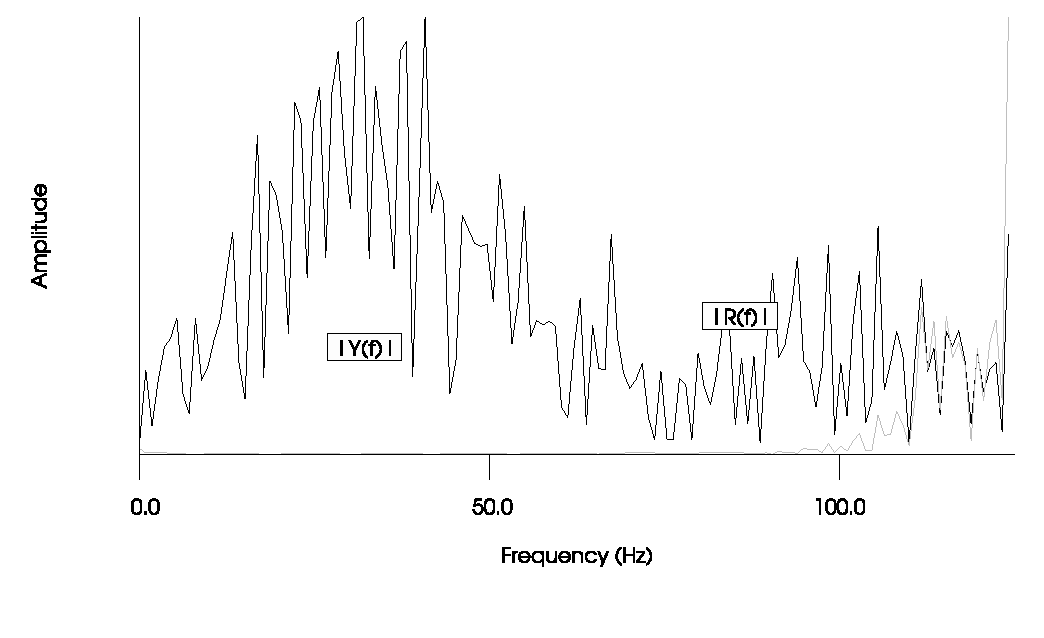
\epsfig{file=Fig/fdecon3-spectr.pdf, width=\textwidth}
\caption{The spectrum of the input data with added noise $|Y(f)+N(f)|$ and the
         deconvolved output $|R(f)|$ (gray line).}
\label{fig:fdecon3-spectr}
\end{figure}
%
\end{frame}
%
\begin{frame}{Deconvolution}
\begin{figure}[h]
%\plot{fdecon3.pdf}{width=\textwidth}{Deconvolution}
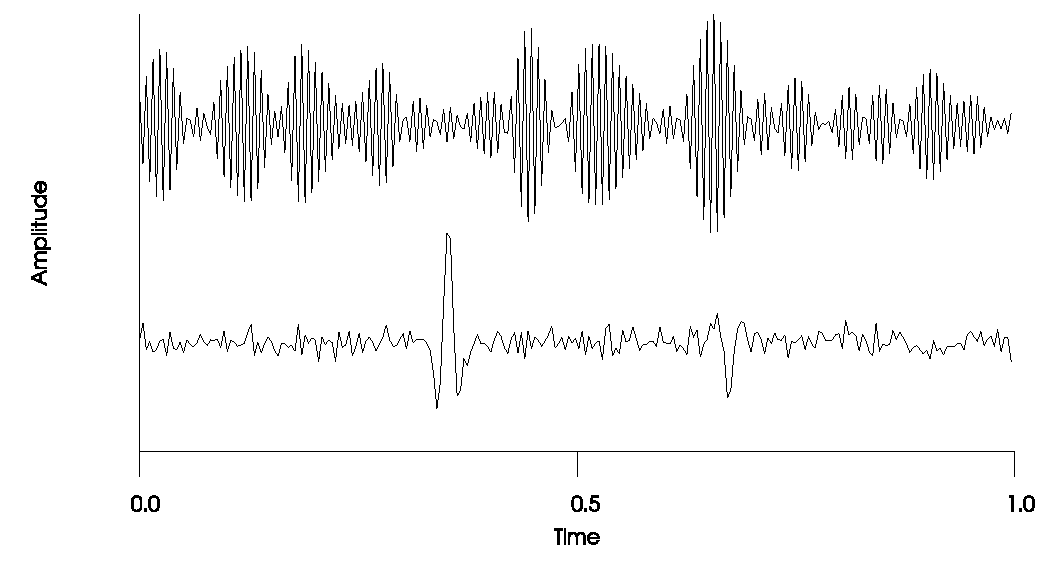
\epsfig{file=Fig/fdecon3.pdf, width=\textwidth}
\caption{The input seismic data with added noise is shown in the lower trace, while the
         ouput of a spiking deconvolution filter applied to the input data
         is shown in the upper trace.}
\label{fig:fdecon3}
\end{figure}
\end{frame}
%
%
\begin{frame}{Deconvolution}
\begin{figure}[h]
%\plot{fig-4-matchspectr.pdf}{width=\textwidth}{Deconvolution}
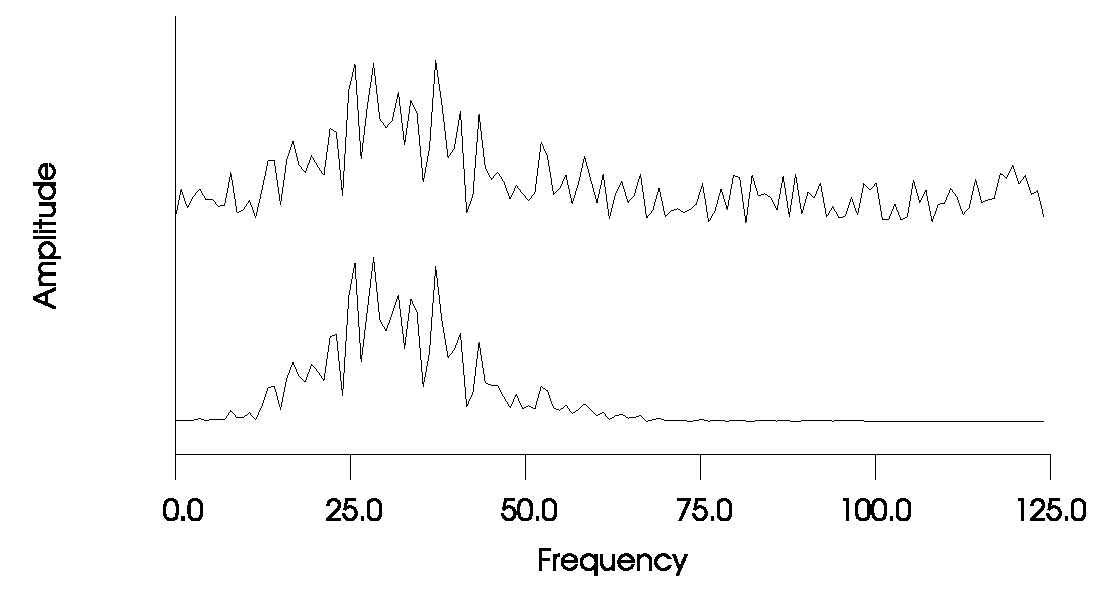
\epsfig{file=Fig/fig-4-matchspectr.pdf, width=\textwidth}
\caption{The spectrum of the input data with added noise $|Y(f)+N(f)|$ and the
         stabilized deconvolved output $|R(f)|$ (gray line).}
\label{fig:fdecon4-spectr}
\end{figure}
\end{frame}
%
%
\begin{frame}{Deconvolution}
\begin{figure}[h]
%\plot{fig-4-matchdecon.pdf}{width=\textwidth}{Deconvolution}
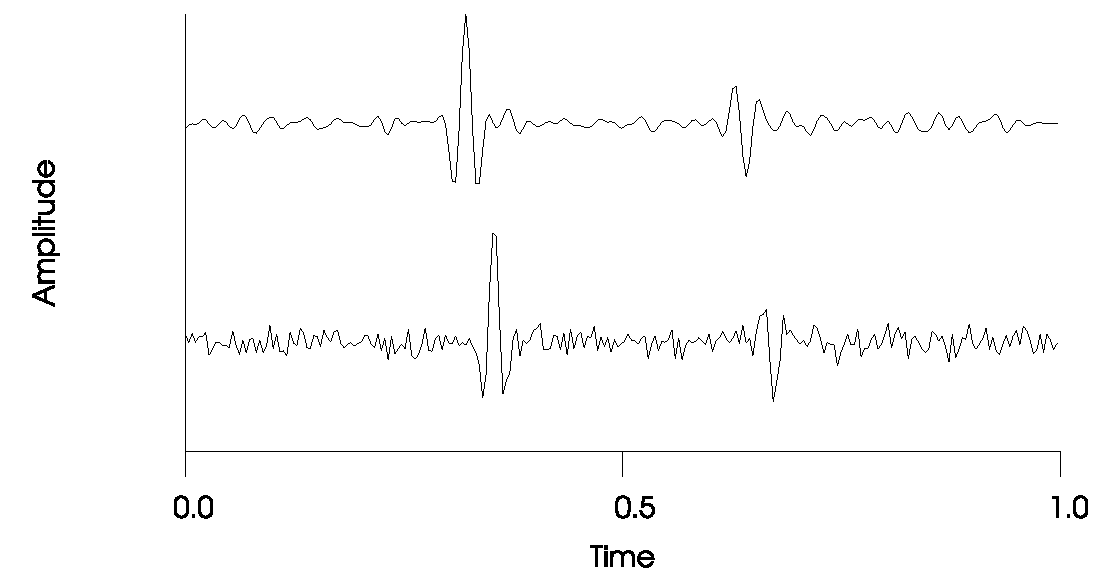
\epsfig{file=Fig/fig-4-matchdecon.pdf, width=\textwidth}
\caption{The input seismic data is shown in the lower trace, while the
         ouput of a match filter applied to the input data
         is shown in the upper trace.}
\label{fig:fdecon4}
\end{figure}
\end{frame}
%----------------------------------------------------------------
%\section{Linear least-squres inversion}
%----------------------------------------------------------------
\begin{frame}{Linear least-squres inversion}
The convolutional model for seismic data
%
\begin{eqnarray}
y(t) = r(t)*s(t),
   \label{eq:inv-convmod}
\end{eqnarray}
%
\begin{itemize}
  \item $y(t)$ : Simulated Seismic data
  \item $r(t)$ : Reflectivity
  \item $s(t)$ : Seismic source pulse
\end{itemize}
$\hat{y(t)}$: Observed seismic data 
\end{frame}
\begin{frame}{Linear least-squres inversion}
%
We want to estimate $r(t)$ by minimizing 
\begin{eqnarray}
  e = \frac{1}{T}\int^{+\infty}_{-\infty}dt\, [\hat{y}(t)-y(t)]^2,
\end{eqnarray}
%
Sampled functions
\begin{eqnarray}
  e = \frac{1}{N}\sum^{N}_{k=0} [\hat{y}_k-y_k]^2.
                       \label{eq:inv-lse}
\end{eqnarray}
%
Inserting equation \eqref{eq:3-64} into equation \eqref{eq:inv-lse} 
%
\begin{eqnarray}
  e = \frac{1}{N}\sum^{N}_{k=0} [\hat{y}_k-\sum^N_{l=0} r_l s_{k-l}]^2.
                       \label{eq:inv-lse2}
\end{eqnarray}
%
\end{frame}
%
\begin{frame}{Linear least-squres inversion}
Minimize error by 
%
\begin{eqnarray}
  \frac{\partial e}{\partial r_m} = 0,
            \label{eq:inv-opt}
\end{eqnarray}
for $m=0,1,2,...,N$.\\
Applying  to equation \eqref{eq:inv-lse2}
%
\begin{eqnarray}
0 = \frac{-2}{N}\sum^N_{k=0}\left[\hat{y}_k-\sum^N_{l=0} s_{k-l} r_l\right] s_{k-m}.
            \label{eq:inv-err2}
\end{eqnarray}
\end{frame}
%
%
\begin{frame}{Linear least-squres inversion}
After reorganizing and multiplication with $-N/2$
%
\begin{eqnarray}
0 = \sum^N_{k=0}\hat{y}_k s_{k-m} - \sum^N_{k=0}\sum^N_{l=0} s_{k-l} s_{k-m} r_l,
            \label{eq:inv-err3}
\end{eqnarray}
%
To simplify introduce the {\em cross correlation}
%
\begin{eqnarray}
  \phi_{\hat{y} s}(m) =\sum^N_{k=0}\hat{y}_k s_{k-m},
             \label{eq:cross-corr}
\end{eqnarray}
and the {\em autocorrelation}
%
\begin{eqnarray}
  \phi_{s s}(m) =\sum^N_{k=0}s_k s_{k-m},
             \label{eq:auto-corr}
\end{eqnarray}
%
Equation \eqref{eq:inv-err3} then becomes
%
\begin{eqnarray}
\phi_{\hat{y} s}(m)= \sum^N_{l=0}\sum^N_{k=0} s_{k-l} s_{k-m} r_l.
            \label{eq:inv-err5}
\end{eqnarray}
% 
\end{frame}
%
\begin{frame}{Linear least-squres inversion}
Make a change of the summation variable
$k'=k-l$ which gives $k=k'+l$
%
\begin{eqnarray}
\phi_{\hat{y} s}(m)= \sum^N_{l=0}\sum^{N-l}_{k'=-l} s_{k'} s_{k'-(m-l)} r_l.
            \label{eq:inv-err6}
\end{eqnarray}
% 
To get
%
\begin{eqnarray}
\phi_{\hat{y} s}(m)= \sum^N_{l=0}\phi_{s s}(m-l) r_l,
            \label{eq:normeq}
\end{eqnarray}
% 
for $m=0,1,,,,N$.
Equation \eqref{eq:normeq} is known as Levinson's {\em normal equations}.
\end{frame}
%
\begin{frame}{Linearized inversion and deconvolution}
%--------------------------------------------------------------
%\section{Linearized inversion and deconvolution}
%--------------------------------------------------------------
Solution of equation \eqref{eq:normeq} corresponds to
deconvolution in the frequency domain given by equation \eqref{eq:refl-noise-eps}
with $\epsilon=0$.
%
\begin{eqnarray}
  \phi_{a b}(t) =\int^{+\infty}_{-\infty} d\tau\, a(\tau)b(\tau-t),
             \label{eq:cross-corr3}
\end{eqnarray}
%
which is the same as
%
\begin{eqnarray}
  \phi_{a b}(t) =\int^{+\infty}_{-\infty} d\tau\, a(\tau+t)b(\tau).
             \label{eq:cross-corr3b}
\end{eqnarray}
%
The last equation is proved by substitution of variables by $u=\tau-t$.

The auto-correlation becomes
%
\begin{eqnarray}
  \phi_{a a}(t) =\int^{+\infty}_{-\infty}d\tau\, a(\tau)a(\tau+t).
             \label{eq:auto-corr3c}
\end{eqnarray}
%
The Fourier transform of equation \eqref{eq:cross-corr3b} is
%
\begin{eqnarray}
  \Phi_{ab}(f)=\int^{+\infty}_{-\infty}dt\, \int^{+\infty}_{-\infty}d\tau\, 
        \exp(-2\pi i f t)a(\tau+t)b(\tau),
\end{eqnarray}
%
\end{frame}
%
\begin{frame}{Linearized inversion and deconvolution}
which becomes after a change of variable $u=\tau+t$:
%
\begin{eqnarray}
  \Phi_{aa}(f)\int^{+\infty}_{-\infty}d\tau\, \left[\exp(2\pi i f \tau)b(\tau)\right]^*
   \int^{+\infty}_{-\infty}du\, \exp(-2\pi i f u) a(u),
\end{eqnarray}
%
which is the same as
%
\begin{eqnarray}
 \Phi_{ab}(f)=A(f)B^*(f). 
             \label{eq:cross-spectr}
\end{eqnarray}
%
If  $a=b$ we get 
%
\begin{eqnarray}
 \Phi_{aa}(f)=A(f)A^*(f) =|A(f)|^2.
             \label{eq:auto-spectr}
\end{eqnarray}
%
The Fourier transform of the auto-correlation is the square of the amplitude spectrum, which
is also called the power spectrum.
\end{frame}
%
\begin{frame}{Linearized inversion and deconvolution}
Fourier-transform equation \eqref{eq:normeq} and use
equations \eqref{eq:cross-spectr} and \eqref{eq:auto-spectr} :
%
\begin{eqnarray}
\hat{Y} S^*(f)= |S(f)|^2 R(f),
            \label{eq:normeq-freq}
\end{eqnarray}
% 
Solving equation \eqref{eq:normeq-freq} for $R(f)$ we get
%
\begin{eqnarray}
R(f) = \frac{\hat{Y(f)}S^*(f)}{|S(f)|^2}
            \label{eq:normeq-freq2}
\end{eqnarray}
% 
which is exactly the same solution as  given by equation \eqref{eq:inv-lse} but with $\epsilon=0$.
\end{frame}
%
\begin{frame}{Linearized inversion and deconvolution}
To stabilize the solution add a damping-constant $\epsilon$ in the error function
given by equation \eqref{eq:inv-lse} 
%
\begin{eqnarray}
  e = \frac{1}{N}\sum^{N}_{k=0} [\hat{y}_k-y_k]^2 +\epsilon\sum^{N}_{k=0}r^2_k.
                       \label{eq:inv-lse-damp}
\end{eqnarray}
%
This gives the normal equations
%
\begin{eqnarray}
\phi_{\hat{y} s}(m)= \sum^N_{l=0}[\phi_{s s}(m-l)+\epsilon\delta_{m,l}] r_l,
            \label{eq:normeq2}
\end{eqnarray}
% 
where the Kronecker symbol $\delta_{m,l}$ is defined as
%
\begin{eqnarray}
\delta_{m,l}=\left\{ \begin{array}{ll}
                       1 & \mbox{$m=l$} \\
                       0 & \mbox{otherwise}\\ 
                     \end{array}
             \right.
\end{eqnarray}
%
A Fourier-transform of equation \eqref{eq:normeq2} gives exactly the
stabilized deconvolution solution in equation \eqref{eq:normeq-freq2}.
\end{frame}
%
\begin{frame}{Predictive deconvolution}
%
\begin{itemize}
\item Predict the input $y_k$ at future time $y_{k+\alpha}$.
\end{itemize}
%
\begin{eqnarray}
  y_{k+\alpha}=\sum^M_{l=0}p_l y_{k-l}. 
                         \label{eq:pred}
\end{eqnarray}
%
\begin{itemize}
  \item Use Wiener filtering
  \item Input: $y_k$ 
  \item Desired output: $y_{k+\alpha}$.
\end{itemize}
\end{frame}
%
\begin{frame}
 \begin{itemize}
  \item Right hand side crosscorrelation:
 \end{itemize}
%
\begin{eqnarray}
  \phi_{y_{k+\alpha}y_k}(m) = \sum^{M}_{l=m} y_{l+\alpha} y_{l-m}.
\end{eqnarray}
%
\begin{itemize}
\item Change of variable $l'=l+\alpha$:
\end{itemize}
%
\begin{eqnarray}
 \phi_{y_{k+\alpha}y_k}(m)  = 
       \sum^{M}_{l'=\alpha+m} y_{l'} y_{l'-(m+\alpha)} = \phi_{yy}(m+\alpha).
\end{eqnarray}
%
\begin{itemize}
\item The normal equations then become
\end{itemize}
%
\begin{eqnarray}
  \sum^M_{l=0} \phi_{yy}(l-m)p_l = \phi_{yy}(m+\alpha), 
                           \label{eq:prednorm}
\end{eqnarray}
%
for $m=0,1,\ldots,M$. 
\end{frame}
%
\begin{frame}
\sf
\begin{itemize}
\item Prediction error
\end{itemize}
%
\begin{eqnarray}
 \epsilon_k = y_{k+\alpha}-\hat{y}_{k+\alpha}.
                 \label{eq:prederr}
\end{eqnarray}
%
\begin{itemize}
\item Prediction error represents  non-predictable part of input data
\item If input data is stationary, white and random with zero mean 
\end{itemize}
% 
\begin{eqnarray}
  \phi_{xx}(m) = 0, \,\, \mbox{for}\,\, m \ne 0\nonumber\\
  \phi_{xx}(m) = \sigma^2. \,\, \mbox{for}\,\, m = 0
\end{eqnarray}
%
\begin{itemize}
 \item Right hand side is zero for nonzero valuesof the prediction distance 
\item Filter coefficients  zero 
\item Predicted value zero, which is mean of input data
\end{itemize}
\end{frame}
%
\begin{frame}{Inverse filters for multiples}
\sf
\begin{itemize}
 \item Replace the predicted value with equation \eqref{eq:pred}
\end{itemize}
%
\begin{eqnarray}
  \epsilon_{k+\alpha}=y_{k+\alpha} -\sum^N_{l=0}p_l y_{k-l}. 
                               \label{eq:prederr2}
\end{eqnarray}
\begin{itemize}
\item $z$-transform of equation \eqref{eq:prederr}
\end{itemize}
\begin{eqnarray}
A(z) = \sum_{k=0}^N a_k z^k
\end{eqnarray}
%
\begin{eqnarray}
  \sum^N_{k=0}z^{k}\epsilon_{k+\alpha}
       =\sum^N_{k=0}z^{k}y_{k+\alpha} -\sum^N_{j=0}z^{k}\sum^N_{l=0}p_l y_{k-l}, 
                               \label{eq:prederr3}
\end{eqnarray}
%
\begin{eqnarray}
  z^{-\alpha}\sum^{N+\alpha}_{m=k+\alpha}z^{m}\epsilon_{m}
       =z^{-\alpha}\sum^{N+\alpha}_{m=k+\alpha}z^{m}y_{m} -\sum^N_{j=0}z^{k}\sum^N_{l=0}p_l y_{k-l}. 
                               \label{eq:prederr4}
\end{eqnarray}
\end{frame}
\begin{frame}{Predictive deconvolution}
%
\begin{eqnarray}
  z^{-\alpha}E(z)
       =z^{-\alpha}Y(z) -P(z)Y(z).
                               \label{eq:prederr5}
\end{eqnarray}
%
\begin{eqnarray}
  E(z)=[1 -z^{\alpha}P(z)]Y(z).
                               \label{eq:prederr6}
\end{eqnarray}
%
\end{frame}
%
\begin{frame}{Predictive deconvolution}
\begin{itemize}
\item The filter
\end{itemize}
%
\begin{eqnarray}
  [1 -z^{\alpha}P(z)],
\end{eqnarray}
\begin{itemize}
 \item Z-transform of the time-domain filter
\end{itemize}
%
\begin{eqnarray}
p_k = 1,0,0,0,0,\ldots,0,-p_0,-p_1,\ldots,-p_N,
                         \label{eq:prederr7}
\end{eqnarray}
%
\begin{itemize}
\item The filter contains $\alpha-1$ zeros. 
\item For $\alpha=1$
\end{itemize}
%
\begin{eqnarray}
p_k = 1,-p_0,-p_1,\ldots,-p_N,
\end{eqnarray}
\begin{itemize}
\item Statistical Wiener spiking deconvolution filter.
\end{itemize}
\end{frame}
%
\begin{frame}{Predictive deconvolution}
%
\begin{figure}[b]
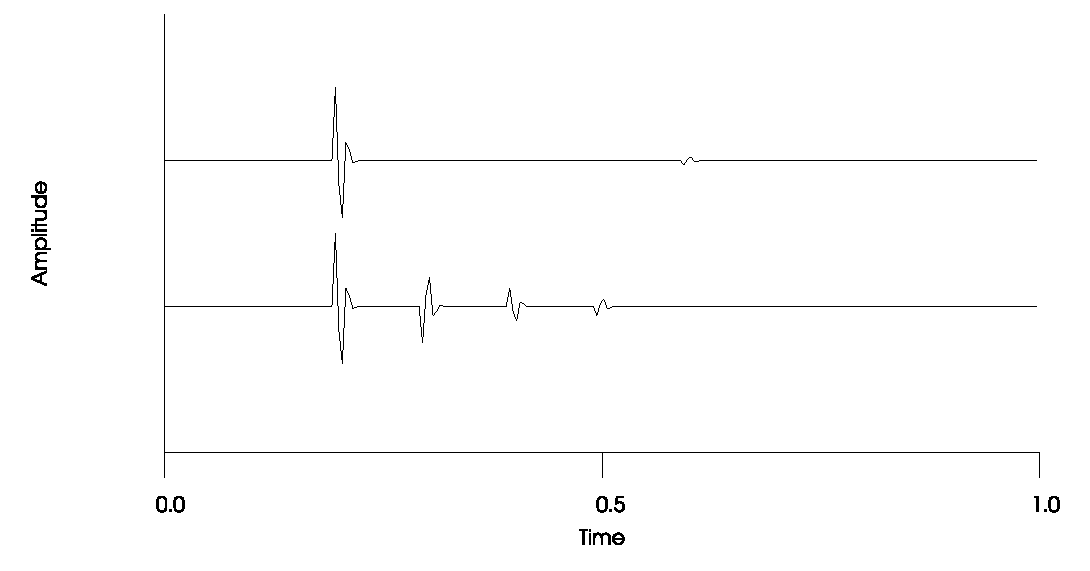
\epsfig{file=Fig/mulre.pdf, width=0.8\textwidth}
\caption{Input seismic data with multiples (lower trace) and output from 
         multiple inverse filter (top)}
\label{fig:mulre}
\end{figure}
\end{frame}
%
\begin{frame}{Predictive deconvolution}
\begin{figure}[h]
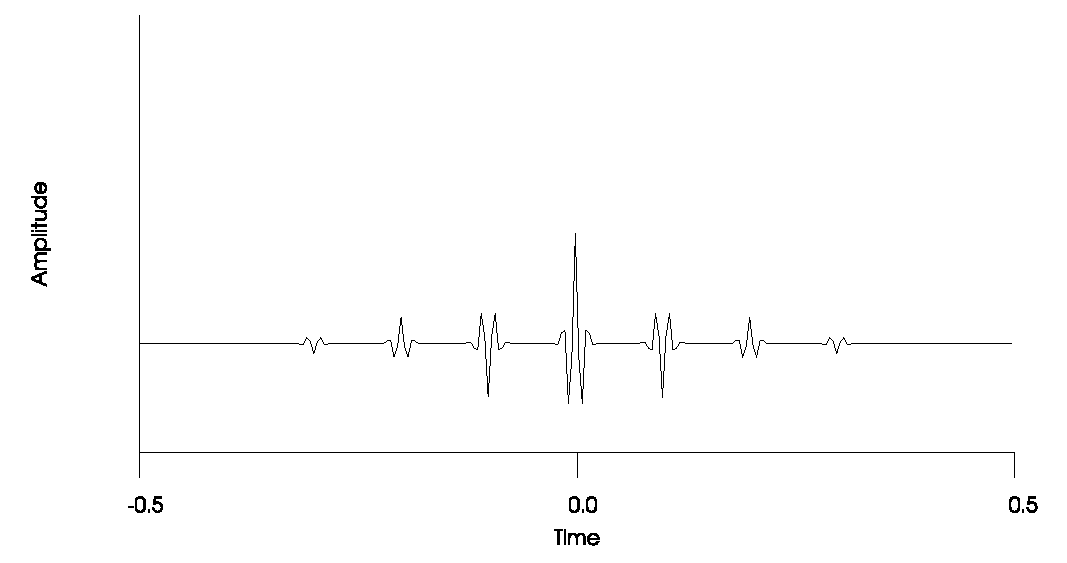
\epsfig{file=Fig/prederr-acorr.pdf, width=0.8\textwidth}
\caption{Autocorrelation of the input data shown in figure \protect{\ref{fig:mulre}}}
\label{fig:prederr-acorr}
\end{figure}
\end{frame}
%
\begin{frame}{Predictive deconvolution}
%
\begin{figure}[h]
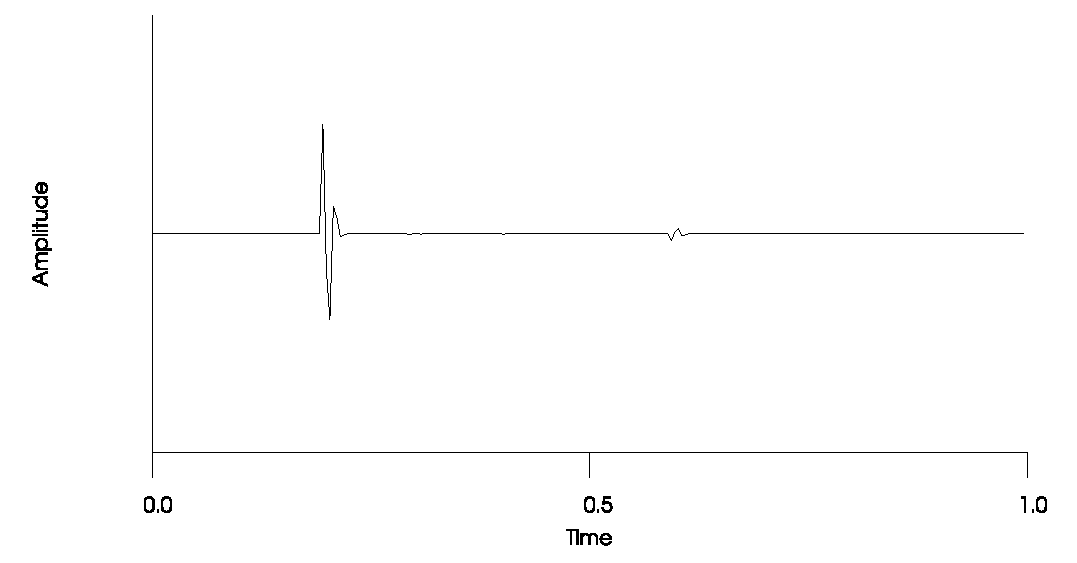
\epsfig{file=Fig/prederr-out.pdf, width=\textwidth}
\caption{Prediction error filter applied to the input data shown in figure \protect{\ref{fig:mulre}}}
\label{fig:prederr-out}
\end{figure}
%
\end{frame}
\begin{frame}{Predictive deconvolution}
%
\begin{figure}[h]
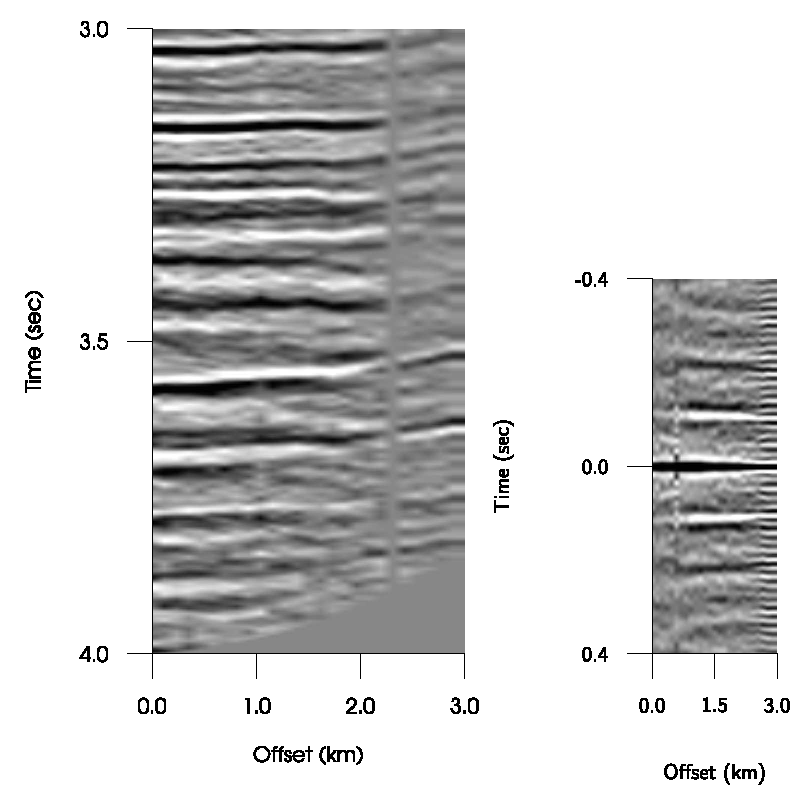
\epsfig{file=Fig/prederr2-acorr.pdf, width=0.6\textwidth}
%\caption{Input CDP gather}
\label{fig:prederr2-cdp}
\end{figure}
\end{frame}
%
\begin{frame}{Predictive deconvolution}
%
\begin{figure}[h]
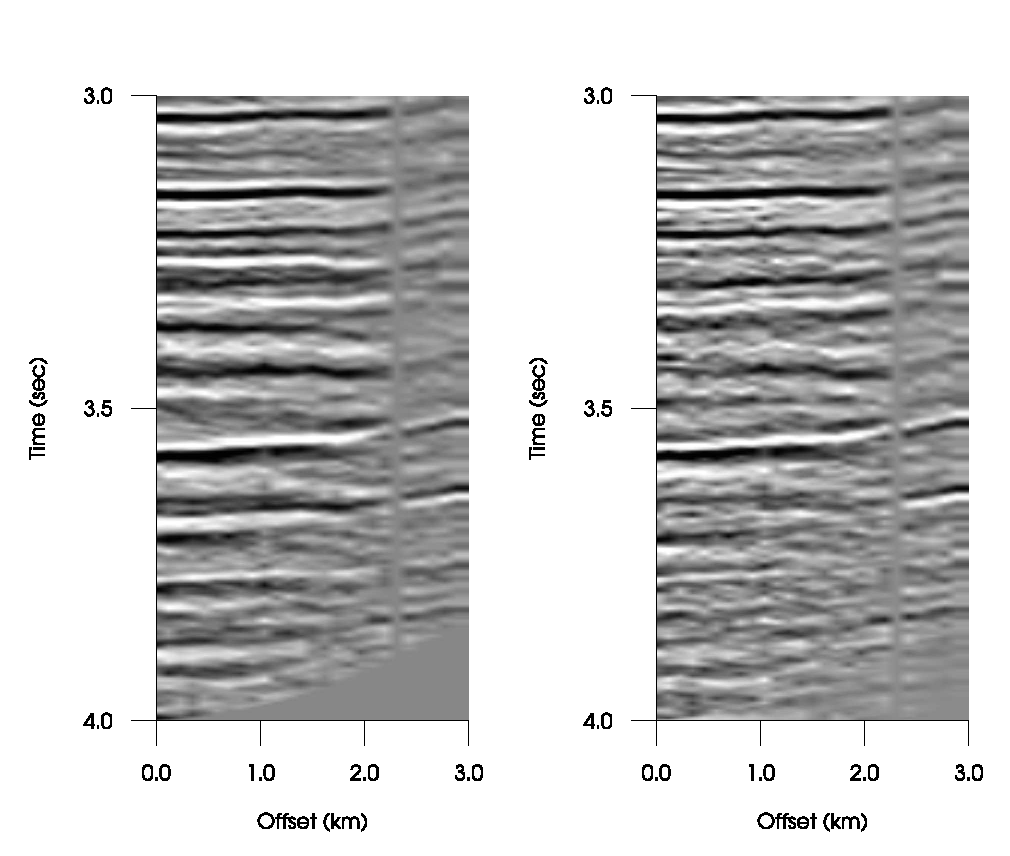
\epsfig{file=Fig/prederr2.pdf, width=0.6\textwidth}
%\caption{Autocorrelation of the CDP gather shown in figure \protect{\ref{fig:prederr2-cdp}}}
\label{fig:prederr2-acorr}
\end{figure}
%
\end{frame}
%
\begin{frame}{Predictive deconvolution}
\begin{figure}[h]
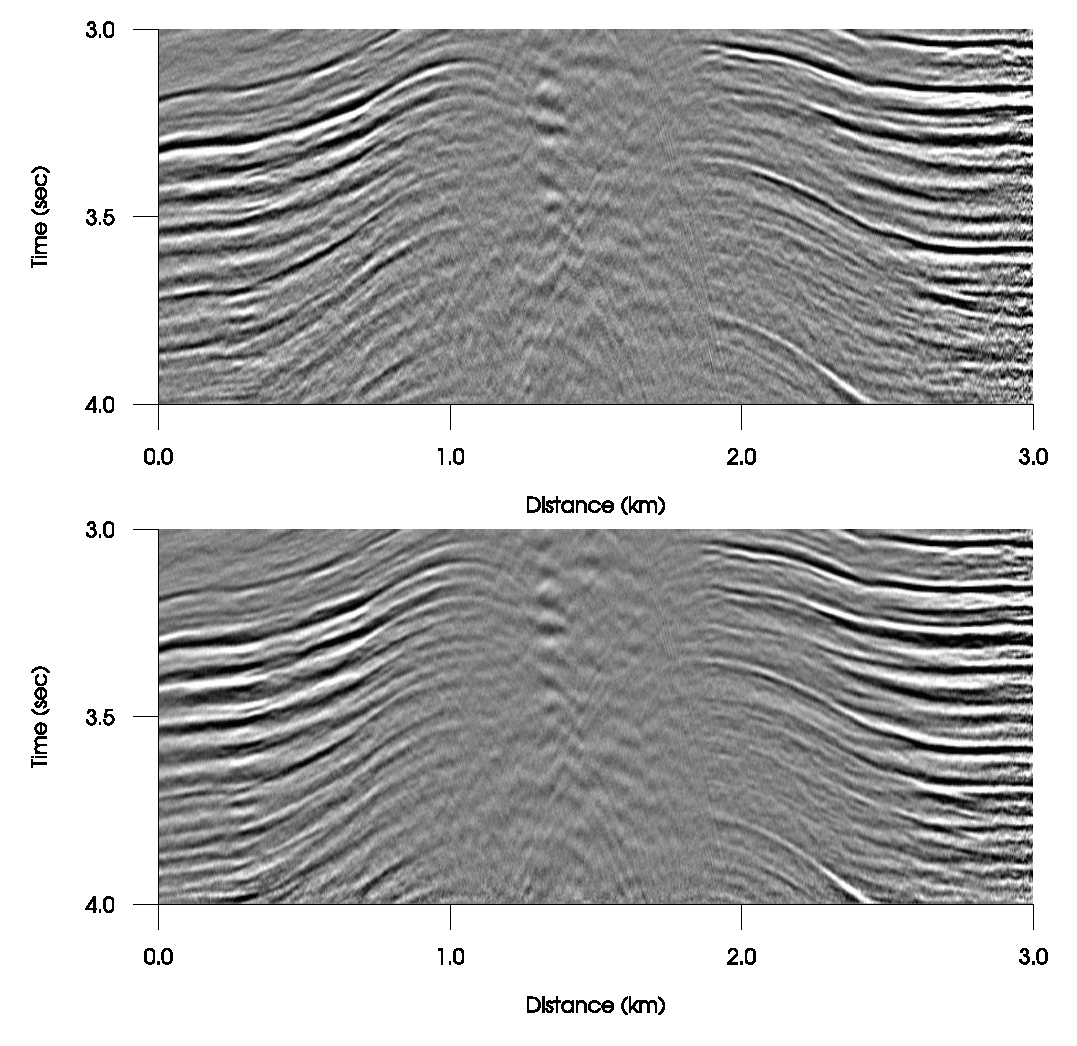
\epsfig{file=Fig/prederr3.pdf, width=0.6\textwidth}
%\caption{Prediction error filter applied to the input CDP gather figure \protect{\ref{fig:prederr2-cdp}}}
\label{fig:prederr3}
\end{figure}
\end{frame}
%
%
\begin{frame}{Predictive deconvolution}
\begin{figure}[h]
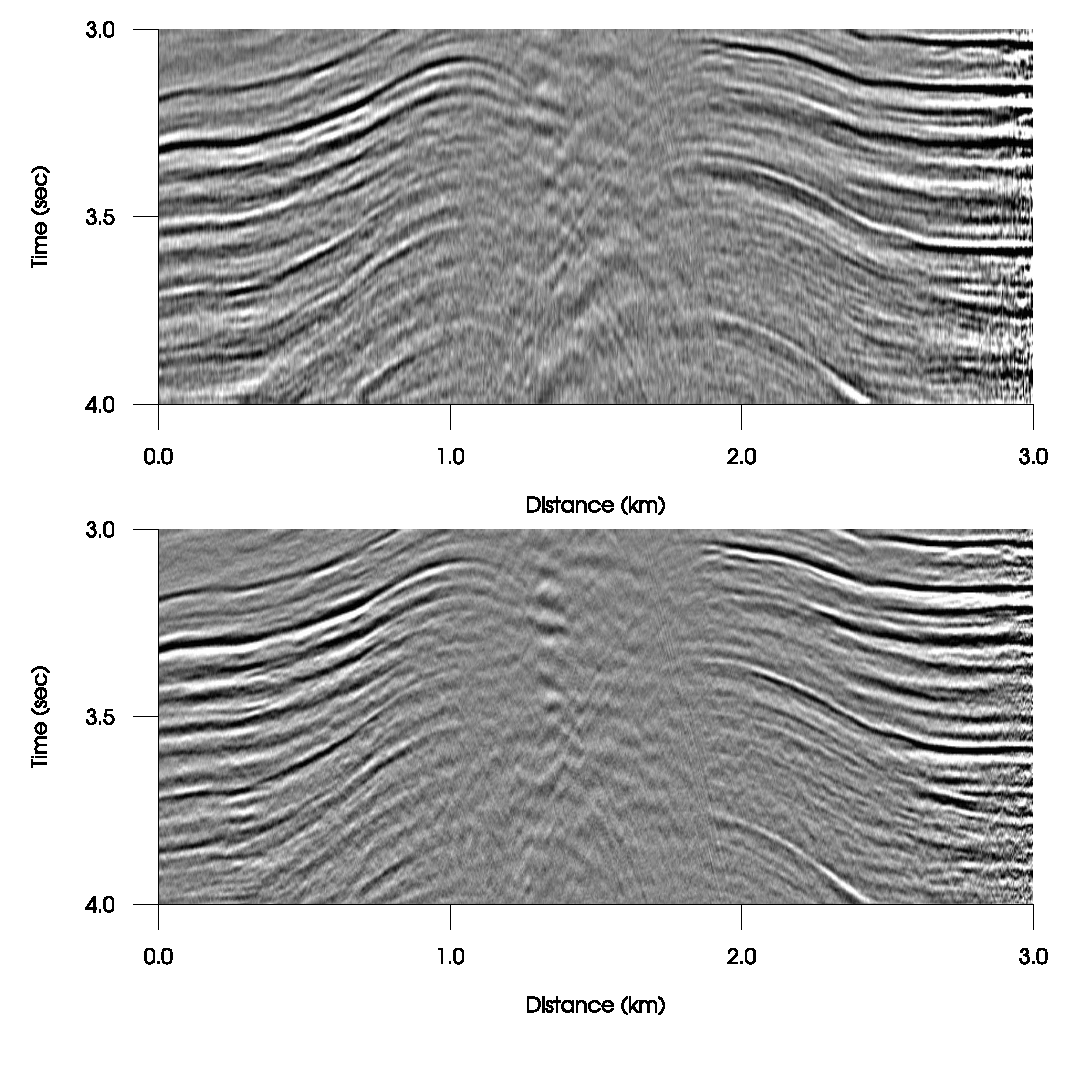
\epsfig{file=Fig/prederr3-spike.pdf, width=0.6\textwidth}
%\caption{Prediction error filter applied to the input CDP gather figure \protect{\ref{fig:prederr2-cdp}}}
\label{fig:prederr3-spike}
\end{figure}
\end{frame}
%
\end{document}
\end{document}
